%定義
本章では,本論文を閲覧するにあたり必要となる用語について述べる.

%1節
\section{スキャンテスト}
スキャンテスト\cite{scantest}とは,組み合わせ回路にFFを取り付けることで,
回路のテストや内部状態の制御・観測を容易にしたテスト手法である.
スキャンテストの構成を図2.1に示す.
\begin{figure}[]
	\begin{center}
		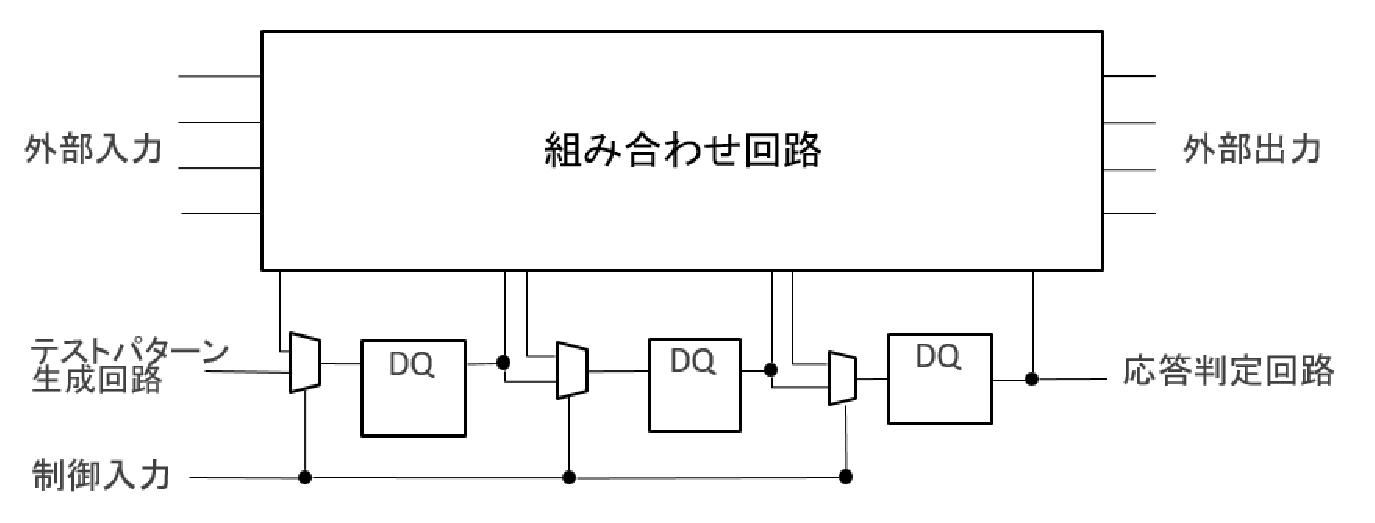
\includegraphics[height=50mm]{scantest.eps}
		\caption{スキャンテスト}
	\end{center}
\end{figure}

対象となる順序回路のFFを,
直列につないだシフトレジスタ(スキャンチェーン)に置き換え,
スキャン出力まで値をシフトし内部状態の制御・観測を行う.
また,テストパターン生成回路とテスト応答判定回路を組込むことで簡易的な検査が可能となる.
テストパターン生成回路には線形帰還シフトレジスタ(LFSR: Linear Feedback Shift Registe)
がよく用いられる.本研究でもLFSRを用いた回路を想定している.
スキャンテストはシフトモードとキャプチャモードによってテストを行う.
シフトモードとは,スキャンインと呼ばれるLFSRが生成したテストパターンを各FFに印加する動作と,
スキャンアウトと呼ばれる結果の出力を行う動作の二つの動作を持つモードである.
キャプチャモードとは,スキャンチェーンに印加したテストパターンを用いて
回路の応答をFFにキャプチャするモードである.

%2節
\section{遅延故障}
論理回路内の素子や信号線における信号変化の伝搬遅延時間が増大し
誤作動を起こす故障を遅延故障\cite{transfault}と呼ぶ.
遅延故障の故障モデルを図2.2に示す.
図に示すように,FFの出力で生じた信号値変化が
組み合わせ回路内を伝搬して次のクロックでFFに取り込まれる際,
遅延時間が決められた範囲を超えることで誤作動が生じる.
遅延故障には,立ち上がり(0から1への変化)の遅延と,
立ち下がり(1から0への変化)の遅延の二通りの故障が考えられる.

\begin{figure}[h]
\begin{center}
	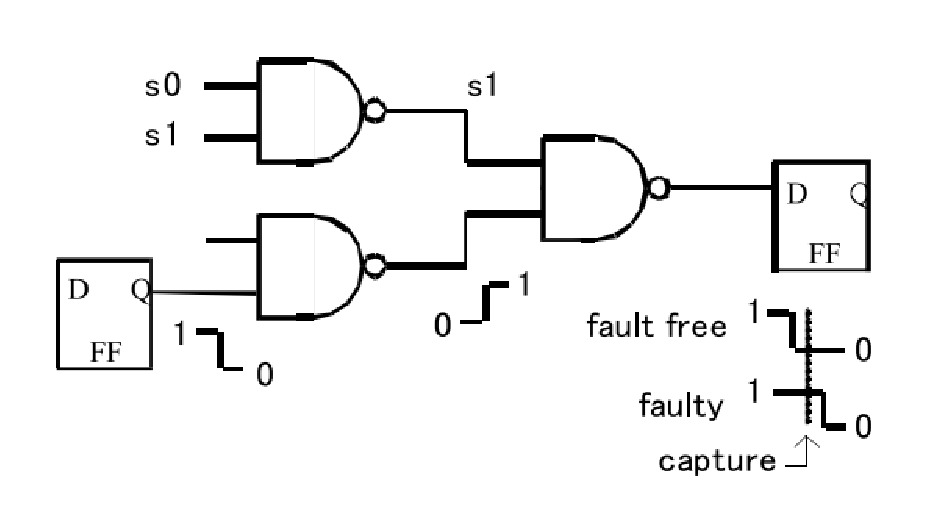
\includegraphics[height=50mm]{transfault.eps}
	\caption{遅延故障モデル}
\end{center}
\end{figure}

%3節
\section{遅延故障のテスト方式}
遅延故障は信号値の変化に起因することから,故障を検出するためには,
変化前の信号値を設定するためのテストパターンと,
変化後の値をキャプチャするためのテストパターンの2つを連続して印加する必要がある.
この手法を2パターンテストと呼ぶ.

2パターンテストで高い故障検出率を得るためには,テストパターンの印加方法を工夫する必要がある.
スキャン動作は,1パターン目の印加と2パターン目の出力の観測に有効であるが、
1パターン目と2 パターン目を連続して実動作時間で印加することができないためである.
この問題を解決する手法の一つとして,次節で説明するラウンチオフキャプチャ方式
(LoC : Launch off Capture)が存在する.

%4節
\section{LoC方式}
LoC方式\cite{transfault}では,スキャンシフト動作で1パターン目をスキャンチェーンに設定した後,
通常動作で, システムクロックにより2パターン目を設定し,続けてキャプチャを行う.
つまり,スキャンインをした後に,システムクロックにより二回キャプチャを行うことになる.
図2.3にクロック信号とスキャンイネーブル信号のタイミングチャートを示す.

\begin{figure}[h]
	\begin{center}
		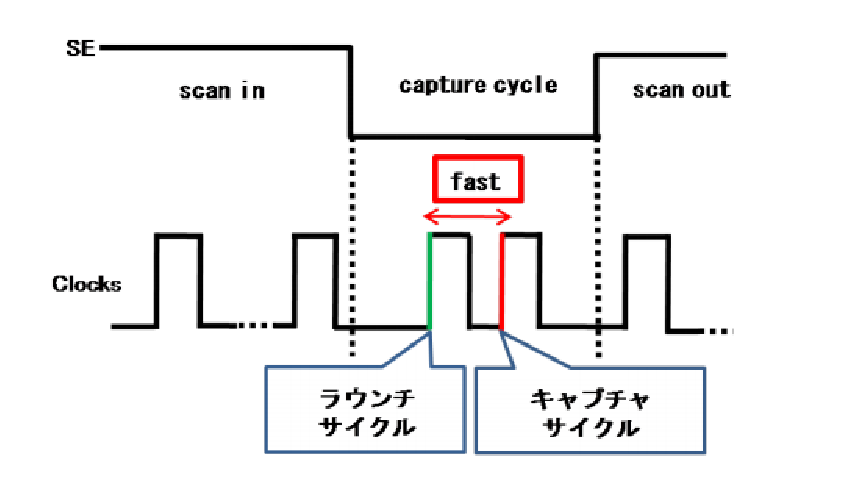
\includegraphics[height=50mm]{LoC.eps}
		\caption{LoCのタイミングチャート}
	\end{center}
\end{figure}

LoC方式の特徴として,2パターン目が通常動作と同じなので設計時の制約が少ないことがあげられる.
また,正常な回路を不良と判定する歩留まりの低下の危険性も少ないこともあげられる.

%本研究では,LoC方式に対して図2.4に示すようにマルチサイクル化を施す.
